\chapter{Experiment No.1: Measuring the bandgap}
\section{Description}
\textbf{Experimental Setup} \\
In this experiment we ought to determine the bandgap of the semiconductors germanium (Ge) and silicon (Si). To reach this goal, we put the semiconductors one after the other in a spectrometer, where the light of a lamp is split up (depending on the wavelengths of the photons making it up) with the help of a lattice. After crossing an aperture slot and a filter, which filters out IR and UV photons, the photons - when reaching the sample - get either absorbed or transmitted, depending on their energy. By measuring the transmission and absorption spectra we can determine the band gap of the sample. \\
\begin{figure}[h]
\begin{center}
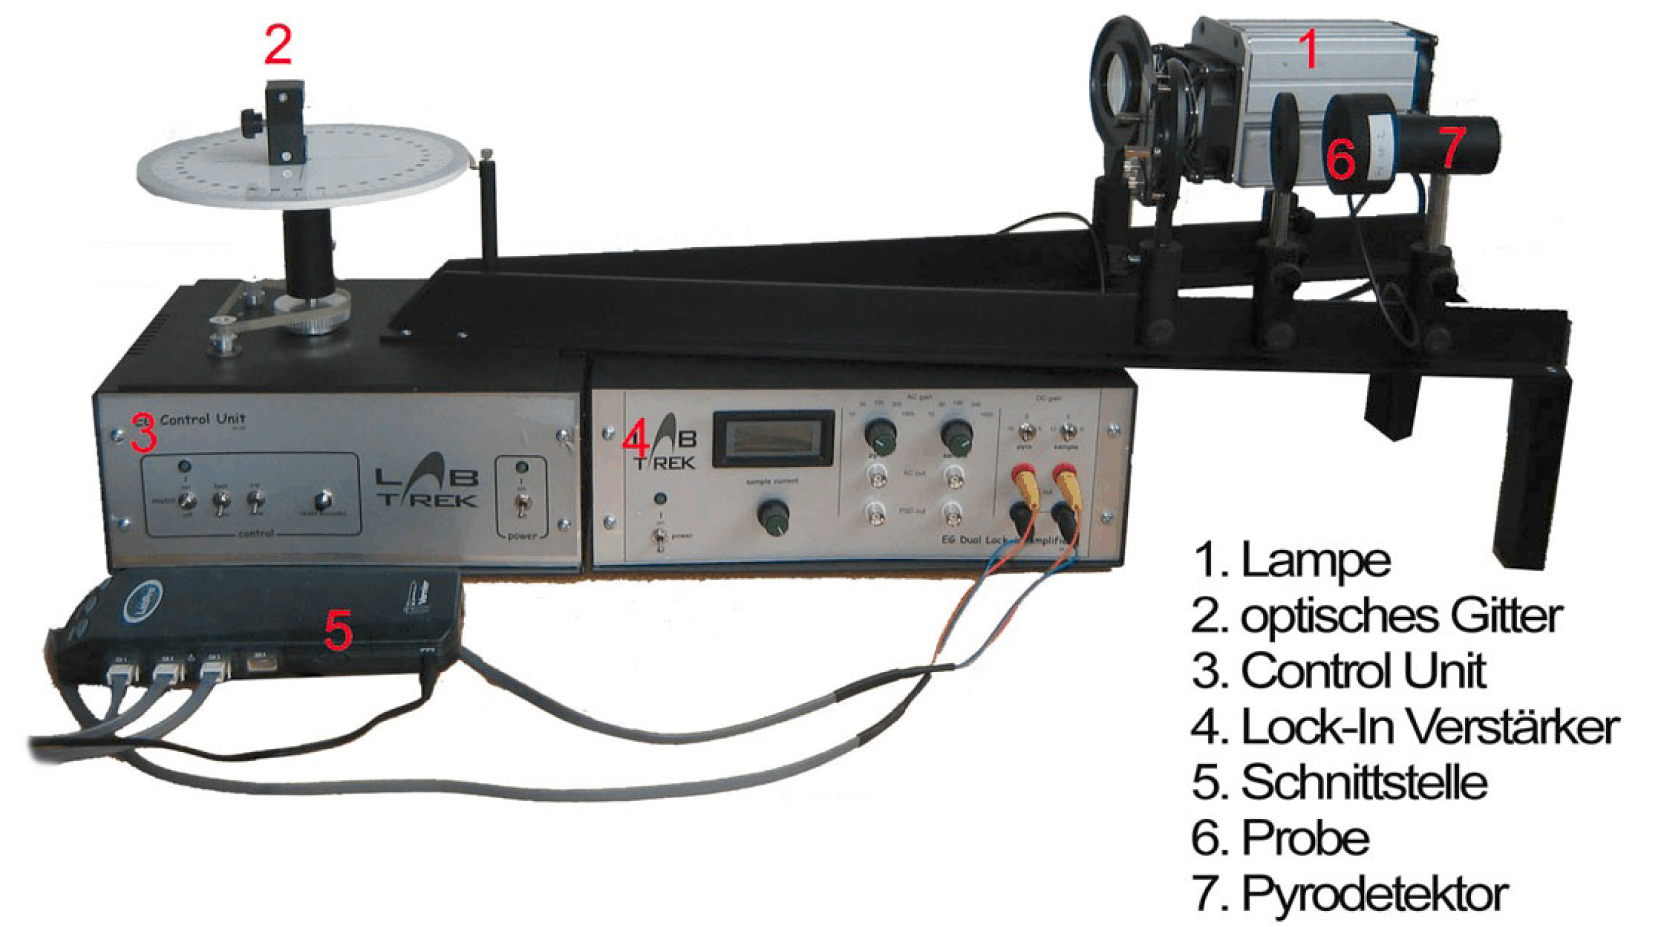
\includegraphics[scale=0.3]{Bilder/Spektrometer.png}\caption{Experimental setup. Source: [Ver]}
\label{spektrometer}
\end{center}
\end{figure}\\
The spectrometer can be seen in the picture above (\ref{spektrometer}). It consists of a lattice (2), which is exposed to light coming from a source (1). There's a chopper right in front of the source, so that the light emitted has a frequency of 70 Hz: that's how the computer can distinguish the source's signals from the signals created by the surrounding light. The 1st order diffraction maximum expands the spectrum: thanks to this, only photons of a specific wavelength (depending on the angle) cross the aperture slit. A small engine helps us measuring the spectra by providing a constant velocity. The absorption in the sample (6) can be measured with the help of the electric current. The transmission spectrum is measured using a pyrodetector (7) connected to a lock-in-amplifier (4), which has the frequency of the chopper as reference signal. \\
Both spectra and the angle (which is measured by the Control Unit(3)) get to the computer via the interface (5).\\
\textbf{Absorption spectrum}\\
Photons with a higher energy than the bandgap energy can excite electrons, so that they move from the valence to the conduction band. Of course this leads to a significant increase in the sample current. If a voltage is applied to the sample, the absorption can be measured with the help of its electric resistance.\\
\\
\textbf{Transmission spectrum}\\
The transmitted photons can be measured with the pyro detector, which detects only changes in the incoming signal. That's why a chopper is applied.\\
\\
\section{Analysis}
To get a transmission and an absorption coefficient, the background has to be substracted from the measured values. The result needs to be divided by the measured value of the source without sample, i.e. the value the pyro detector measures. The formulas for the spectra are the following:\\
\\
$Trans_{real}=\frac{Trans_{measured}-Background}{Lightsource}$\\  
\\                         $Absorp_{real}=\frac{Absorp_{measured}-Background}{Lightsource}$\\
\\
To determine the bandgap energy, we plotted the transmission and absorption spectra over the energy and did linear fits at the flanks of the curves. The intersection point of these linear fits with the horizontal lines through the maximum of the transmission spectrum (for the transmission) and the minimum of the absorption spectrum (for the absorption) provide us with a maximum and a minimum value of the bandgap energy. As we calculated the intersection points for both "negative" (because in the formula for the energy we have $E\propto\frac{1}{sin\theta}$) and positive energies, we get four values for each sample.\\
The energy and its error were calculated as follows:\\
$m*E+c=d$\\
$\Leftrightarrow E=\frac{d-c}{m}$\\
$\Rightarrow s_{E}=\sqrt{(\frac{\partial{E}}{\partial{d}})^2*s_{d}^2+(\frac{\partial{E}}{\partial{c}})^2*s_{c}^2+(\frac{\partial{E}}{\partial{m}})^2*s_{m}^2}=\sqrt{\frac{s_{d}^2}{m^2}+\frac{s_{c}^2}{m^2}+\frac{(d-c)^2}{m^4}*s_{m}^2}$\\
\\
The results are the following:\\
\begin{table}[htbp]
  \centering
  \caption{Results}
    \begin{tabular}{rrrrr}
    $Sample$ & $E_{trans}$  & $s_{E_{trans}}$ & $E_{absorp}$ & $s_{E_{absorp}}$ \\
    Si    & -1,10  & 0,08  & -1,08 & 0,03 \\
    Si    & 1,11  & 0,04  & 1,04  & 0,03 \\
    Ge    & -0,64 & 0,06  & -0,65 & 0,08 \\
    Ge    & 0,63  & 0,05  & 0,63  & 0,04 \\
    \end{tabular}%
  \label{tab:addlabelx}%
\end{table}%
\\
All results are in eV. The plots are in the appendix. \\
Using these results, the weighted mean was calculated as follows (with the "negative" energies being positive in this calculation):\\
$\overline{E_{Si}}=\sum_{i=1}^{4}\frac{\frac{E_{i}}{s_{i}^2}}{\frac{1}{s_{i}^2}}}=1,087 eV$\\
$s_{\overline{E_{Si}}}=\sqrt{\frac{1}{\sum_{i=1}^{4}s_{i}^2}}=0,018 eV$\\
\\
The same equations hold for Ge too.\\
$\Rightarrow \overline{E_{Ge}}=(0,64\pm0,03) eV$\\
\\
The literature values given in [Ver] were $E_{Si}=1,12 eV$ and $E_{Ge}=0,66 eV$.\\
Our results are two(for Si) and one (for Ge) root-mean-square errors from the respective literature values. This is a good result, especially regarding the fact, that the calculations for the absorption and transmission coefficients had to be made without having measured values for both sample and source at the same angle. Of course the difference of the angles is really small, still, it's not necessarily 0: for that reason we have a systematic error in this part of the experiment. Also, we didn't have any errors given on parts of our spectrometer such as the interface, the cables, the pyrodetector, the lock-in-amplifier or the Control Unit. Another errors might have resulted from not taking into account the width of the aperture slit and the effect of the clearly visible fingerprint on the lattice in the Si-experiment.\\
\\
We can state that the error is too low on our results. Still, they are very close to their respective literature values, making the negligence of the errors listed above seem reasonable.


